%!TEX root = ./main.tex
\section{Waves and Diffusion}
\subsection{The wave equation}
Recall that the wave equation in in dimension
\[ u_{tt} = c^2 u_{xx} \quad \mathrm{for} \quad -\infty < x,t < \infty\]
Observe that
\[ 0 = u_{tt} - c^2 u_{xx} = \left( \frac{\partial }{\partial t} - c \frac{\partial }{\partial x} \right) \left( \frac{\partial }{\partial t} + c \frac{\partial }{\partial x} \right)v  =: v \]
We can equivalently write our second order PDE as 
\[\left\{ \begin{array}{rl} 
	u_{t} + c u_{x} &= v \quad (2) \\
	v_t - c v_x &= 0 \quad (1) \\
\end{array} \right. \]
We know that the general solution to (1) is
\[ v(x,t) = h(x + ct)\]
where $h$ is an arbitrary function of one variable. Then substituting $v$ into (2) gives us
\[ u_t + cu_x = h(x + ct)\]
We know that one particular solution is given by $u(x,t) = f(x,t)$, where 
\[ f'(s) = \frac{h(s)}{2t}\]
To that, we can add any of the homogeneous solution
\[ u_t + c u_x = 0 \implies u(x,t) = f(x + ct) + g(x - ct)\]
Hence we have shown that 
\[ u(x,t) = f(x + ct)  - g(x - ct)\]
where $f,g$ are arbitrary function.
\subsubsection{Characteristic coordinates}
Take
\[ \xi = x + ct \qquad \eta = x - ct\]
By the chain rule we have
\[ \partial_x = \frac{\partial}{\partial x} = \frac{\partial }{\partial \xi} \frac{\partial \xi}{\partial x} + \frac{\partial }{\partial \eta} \frac{\partial \eta}{\partial x} = \partial_\xi + \partial_\eta\]
\[ \partial_t = \frac{\partial}{\partial t} = \frac{\partial }{\partial \xi} \frac{\partial \xi}{\partial t} + \frac{\partial }{\partial \eta} \frac{\partial \eta}{\partial t} = c\partial_\xi - c\partial_\eta \]
Hence
\[ \partial_t - c \partial_x = -2c \partial_\eta \qquad \partial_t + c \partial_x = 2c \partial_\xi\]
SO the wave equation is of the form
\[ 0 = (\partial _t - c\partial_x)(\partial_t + cd_x)u = (-4c \partial_\xi)(2c\partial_\eta)u = -4c^2\partial u_{\xi \eta}\]
Since $-4c^2 \neq 0$, we have $u_{\xi \eta} = 0$.
So $u(x,y) = f(\xi) + g(\eta)$.
\subsubsection{Initial Value Problem}
Take 
\[ \left\{ \begin{array}{rl} 
	u_{tt}  &= c^2 u_{xx}   \\
	u(x,0) &= \phi(x) \\
	u_t(x,0) &= \psi(x)
\end{array} \right. \]
where $\phi(x) = \sin x$, and $\psi(x) = 0$.
From the general solution we put $t = 0$ and obtain.
\[ \phi(x) = f(x) + g(x)\]
differential by $t$ we get
\[ \psi(x) = cf'(x) - cg'(x)\]
differentiate $\phi$ and divide $\psi$ by $c$ we get
\[ \phi's = f' + g' \qquad \frac1c \psi = f' - g'\]
Solving for $f'$ and $g'$ gives us
\[ f' = \frac 12 \left( \phi' + \frac \psi c \right) \qquad g' = \frac 12 \left( \phi' - \frac \psi c \right)  \]
Integrate with respect to $s$ gives us
\[ f(s) = \frac 12 \phi(s) + \frac 1{2c} \int_0^s \psi + A \qquad f(s) = \frac 12 \phi(s) - \frac 1{2c} \int_0^s \psi + B\]
where $A,B$ are constants. Since $\phi(x) = f(x) + g(x)$, we have $A + B = 0$. Let $s = x + ct$ and $s = x - ct$ we get
\[u(x, t)=\frac{1}{2} \phi(x+c t)+\frac{1}{2 c} \int_{0}^{x+c t} \psi+\frac{1}{2} \phi(x-c t)-\frac{1}{2 c} \int_{0}^{x-c t} \psi\]
which is reduced to 
\[ \boxed{u(x,t) = \frac12 \left[ \phi(x + ct) + \phi(x - ct) \right] + \frac 1 {2c} \int_{x - ct}^{x + ct} \psi(s) d(s)}\]
\begin{example}
	Take $\phi = 0$ and $\psi = \cos x$. Solve for the wave equation.
\end{example}

\subsection{Causality and Energy}
{\huge TODO}

\subsubsection{The Diffusion Equation}
\begin{problem}
	We want to study the behavior of \[ u_t = ku_{xx}.\]
\end{problem}
\begin{theorem}[The Maximum Principle]
	If $u(x,t)$ that satisfies the diffusion equation in a rectangle $(0 \leq x \leq l, o \leq t \leq T)$.
	\begin{center}
		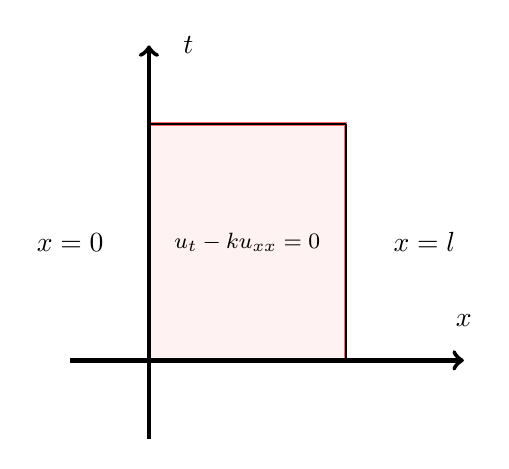
\begin{tikzpicture}
			\filldraw[color=red!60, fill=red!5, very thick] (0,0) -- (2.5,0) -- (2.5,3) -- (0,3) -- (0,0);
			\draw[->, ultra thick] (-1,0) -- (4,0);
			\draw[->, ultra thick] (0,-1) -- (0,4);
			\node at (4,0.5) {$x$};
			\node at (0.5,4) {$t$};
			\draw[thick] (2.5,0) -- (2.5,3);
			\draw[thick] (0,3) -- (2.5,3);
			\node at (-1,1.5) {$x = 0$};
			\node at (3.5,1.5) {$x = l$};
			\node at (1.25, 1.5) {\footnotesize $u_t - ku_{xx} = 0$};
		\end{tikzpicture}
	\end{center}
	then the maximum value of $u(x,t)$ is assumed either initially at $t = 0$ or on the lateral bounding at $x = 0$ or $x = l$.
\end{theorem}
\begin{remark}
	\begin{enumerate}
		\item This is called the \textbf{weak} maximum principle. The \textbf{strong} maximum principle asserts that the maximum value of $u$ cannot occur in the interior (unless $u$ is constant)
		\item The same results hold for minimum (simple solve for $-u(x,t)$ will show).
		\item The are no `hot spots'
	\end{enumerate}
\end{remark}
\begin{proof}[Idea of the proof]
	By contradiction, we want to assume that $u$ attains it maximum value at an interior  $(x_0, t_0)$. Then by calculus at $(x_0, t_0)$ we have
	\[ u_t = 0, \quad u_x = 0, \quad u_{xx} \leq 0\]
	If we know that $u_{xx}(x_0, t_0) \neq 0$ then $u_{xx} (x_0 ,t_0) \leq 0$, so $u_{t} - k u_{xx} > 0$. A contradiction.
\end{proof}
\begin{proof}
	The $M$ denote the maximum of $u$ on the rectangle. We want to show $u \leq M$ for all points $(x_0,t_0)$ in rectangle. Let $\varepsilon > 0$ be fixed, and define 
	\[ v(x,t) := u(x,t) + \varepsilon x^2\]
	\textit{Goal:} Show $v(x,t) \leq M + \varepsilon l^2$ in $\b R$. This is enough since the equation above will imply $u(x,t) \leq M + \varepsilon (l^2 - x^2)$ in $\b R$. As this holds for any $\varepsilon > 0$, this implies $u(x,t) \leq M$ in $\b R$. \\
	We have two things to do
	\begin{enumerate}
		\item Note that on the rectangle $u(x,t) \leq M + \varepsilon l^2$. 
		\item $v$ satisfies the diffusion inequality
		\[ u_t - ku_xx = \underbrace{u_t - ku_{xx}}_{ = 0 \,\, \text{by def. of } u} - 2 \varepsilon k = -2\varepsilon k < 0.\]
		\item \begin{enumerate}
			\item Now suppose for a contradiction that $v(x,t)$ attains its maximum value at an \textbf{interior} point $(x_0, t_0)$ o f$\b R$. i.e,
			\[ 0 < x_0 < l \quad \mathrm{and} \quad 0 < t_0 < T\]
			By calculus at $(x_0, t_0)$ we have
			\[ v_t = 0, \quad v_x = 0, \quad v_{xx} \leq 0.\]
			Hence at $(x_0, t_0)$
			\[ v_t - kv_{xx} = o - kv_{xx} \geq 0,\]
			a contradiction.
			\item Suppose $u$ attain its maximum at final time, the top edge of $\b R$. 
			\[ 0 < x_0 < l \quad \mathrm{and} \quad t_0 = T\]
			Then again by calculus at $(x_0, t_0)$ we have $v_t \geq 0, v_x = 0, v_{xx} \leq 0$. Hence $v_t - k v_{xx} \geq 0$, a contradiction.
		\end{enumerate}

	\end{enumerate}
\end{proof}
\begin{theorem}
	Given set of $,f,g,h, \phi$, there exists at most one solution of
	\[ \left\{ \begin{array}{rl} 
		u_t - k u_{xx} &= f(x,t) \quad \mathrm{for} \,\, 0 < x < l, t > 0 \\
		u(x,0) &= \phi(x)  \\
		u(0,t) &= g(t) \\
		u(l,t) &= h(t)
	\end{array} \right. \]
\end{theorem}
\begin{proof}
	Let $u_1,u_2$ be two solutions of $f,g,h, \phi$. We want to show that $u_1=  u_2$. Define $w := u_1 - u_2$. Then
	\[ \left\{ \begin{array}{rl} 
		w_t - k w_{xx} &= f(x,t) \quad \mathrm{for} \,\, 0 < x < l, t > 0 \\
		w(x,0) &= \phi(x)  \\
		w(0,t) &= g(t) \\
		w(l,t) &= h(t)
	\end{array} \right. \]
	Let $T > 0$, then by the maximum principle 
	\[ w(x,t) \leq 0 \quad \text{for all} \quad 0 < x < l, 0 < t <T.\] Also by the maximum principle
	\[ w(x,t) \geq 0\]
	so $w(x,t) = 0$ for all $0 < x < l, 0 < t< T$. Since $T > 0$ is arbitrary, $u_1 = u_2$.
\end{proof}
	Given $f,g,h, \phi_1, \phi_2$,and suppose $u_1, u_2$ solves the diffusion equation with respect with $\phi_1$ and $\phi_2$ thne
	\[ \max_{0 \leq x \leq l} \left| u_1(x,t) - u_2(x,t)\right| \leq \max_{0 \leq x \leq l} \left| \phi(x) - \phi_2(x)\right| \quad \forall t > 0.\]
\end{theorem}
\begin{proof}
	{\huge TODO}
\end{proof}